\Chapter{Functions}
\Lettrine[loversize=0.1,nindent=0pt]{Picture} a machine that takes in inputs and produces outputs. It could, for instance, double every number put into it. It may return the sum of all of its inputs, the product of all its inputs, or the largest number among all the inputs. That is what a function is -- a relation that maps inputs to outputs. It is this kind of particular relation that we look at in this chapter.

\section{What is a Function?}
\begin{definition}[Function]
    A \term{function}\index{function} $f$ from a set $X$ to a set $Y$ is a relation from $X$ to $Y$ satisfying two properties.
    \begin{enumerate}[label=\textbf{F\arabic*.},leftmargin=1.35\parindent]
        \item $\forall x \in X, \exists y \in Y \text{ s.t. } (x \mathrel{f} y)$
        \item $\forall x \in X, \forall y_1, y_2 \in Y, (((x \mathrel{f} y_1) \land (x \mathrel{f} y_2)) \implies (y_1 = y_2))$
    \end{enumerate}
    We denote such a function by $f: X \to Y$.
\end{definition}

The condition \textbf{F2} essentially says that if a single $x \in X$ is related to two (or more) elements in $Y$, then they must be equal. This can be thought of as the ``uniqueness'' property of a function.

We can succinctly write both \textbf{F1} and \textbf{F2} in one statement using the \term{uniqueness quantifier}\index{uniqueness quantifier}\index{quantifier!uniqueness} $\exists!$. A statement of the form $\exists! x \text{ s.t. } P(x)$, where $P(x)$ is a predicate, is logically equivalent to the statement
\[
    \exists x \text{ s.t. } (P(x) \land (\forall y (P(y) \implies x = y))),
\]
i.e. there exists an $x$ that satisfies the predicate and any $y$ satisfying the predicate must be equal to $x$. Thus, we can combine \textbf{F1} and \textbf{F2} into the single condition
\[
    \forall x \in X, \exists! y \in Y \text{ s.t. } x \mathrel{f} y.
\]
This formulation of the function condition is what we will be using most of the time.

As mentioned, we may think of a function as a machine or process that takes in inputs and produce outputs. In particular, the `machine' for the function $f: X \to Y$ is a machine that \textbf{must} produce an output for any valid input (i.e., an input that comes from $X$) that is provided to it, and it must produce the same output for the same input that is provided to it.

\begin{figure}[H]
    \centering
    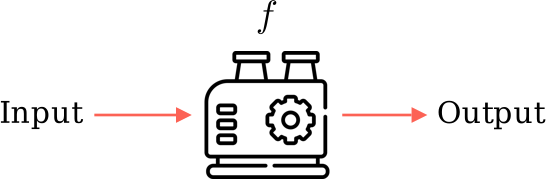
\includegraphics[height=2cm]{images/part-1/functions/function-as-machine.png}
    \caption{Function as a Machine}
\end{figure}

Since there is only one output for any given input, we can denote it unambiguously.

\begin{definition}[Image of an Element Under a Function]\label{definition:image-of-element-under-a-function}
    Let $X$ and $Y$ be sets and $f: X \to Y$ be a function. Suppose $x \in X$. The unique element of $Y$ that is related to $x$ under $f$ is called the \term{image of $x$ under $f$}\index{image!of an element}\index{function!image!of an element} and is denoted $f(x)$.
\end{definition}

Let us look at some examples.

\begin{example}[The Successor Function]
    Let's look at a function that we already looked before, the successor function. Before, we defined it for sets. We can restrict it to the natural numbers. That is, the function $S: \N \to \N$ is defined by $S(n) = n \cup \{n\}$ (remember, we use the counter set for any natural number $n$).
    \begin{figure}[H]
        \centering
        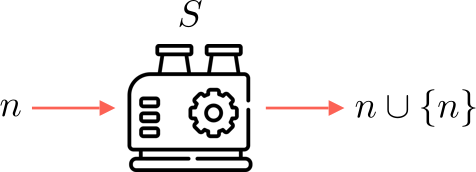
\includegraphics[height=2cm]{images/part-1/functions/successor-as-machine.png}
        \caption{Successor Function as a Machine}
    \end{figure}
\end{example}

\begin{example}[The Identity Function]
    Let $A$ be a set. The identity function $\id_A: A \to A$ is the function such that $\id_A(x) = x$ for all $x \in A$. That is, this function does not transform the input into it in any way.
    \begin{figure}[H]
        \centering
        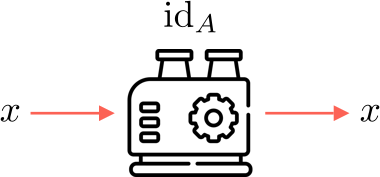
\includegraphics[height=2cm]{images/part-1/functions/identity-as-machine.png}
        \caption{Identity Function as a Machine}
    \end{figure}
    Let us look at some examples of images under the identity function. Suppose $A = \{1, 2, 3\}$. Then
    \begin{itemize}
        \item $\id_A(1) = 1$;
        \item $\id_A(2) = 2$; and
        \item $\id_A(3) = 3$.
    \end{itemize}
\end{example}

\begin{exercise}[Empty Function?]
    Suppose $A$ is a set. Consider the relation $f$ from $\emptyset$ to $A$ where $f = \emptyset$. Is $f$ a function?
\end{exercise}

Let's now turn our attention to determining the equality of two functions. Recall that two relations $R$ and $S$ from the set $A$ to the set $B$ and the set $C$ to the set $D$ respectively (i.e., $R \subseteq A \times B$ and $S \subseteq C \times D$) are equal if and only if $A = C$, $B = D$, and $R = S$ as sets (\myref{definition:equality-of-relations}). Since functions are also relations, this definition applies to functions.

\begin{definition}[Equality of Functions]\index{function!equality}
    Let $A$, $B$, $C$, and $D$ be sets. The functions $f: A \to B$ and $g: C \to D$ are equal, denoted $f = g$, if and only if $A = C$, $B = D$, and $f = g$ as sets.
\end{definition}

However, we have a more applicable result for functions.
\begin{theorem}[Equality of Functions, More Easily]
    Let $A$, $B$, $C$, and $D$ be sets. Let the functions $f: A \to B$ and $g: C \to D$. Then $f = g$ if and only if $A = C$, $B = D$, and $f(x) = g(x)$ for all $x \in A$.
\end{theorem}
\begin{proof}
    For the forward direction, suppose $f = g$ (as functions). Thus $A = C$, $B = D$, and $f = g$ as sets. Suppose $x \in A$ and $y \in B$ are arbitrary. Note
    \begin{align*}
        & y = f(x)\\
        \iff& (x, y) \in f & (\myref{definition:image-of-element-under-a-function})\\
        \iff& (x, y) \in g & (\text{as } f = g \text{ as sets})\\
        \iff& y = g(x) & (\myref{definition:image-of-element-under-a-function})
    \end{align*}
    which means $f(x) = g(x)$ for any $x \in A$.

    For the reverse direction, suppose $A = C$, $B = D$, and $f(x) = g(x)$ for all $x \in A$. Then
    \begin{align*}
        & (x, y) \in f\\
        \iff& y = f(x) & (\myref{definition:image-of-element-under-a-function})\\
        \iff& y = g(x) & (\text{as } f(x) = g(x)\;\forall x \in A)\\
        \iff& (x, y) \in g & (\myref{definition:image-of-element-under-a-function})
    \end{align*}
    which means that $f = g$ as sets. Thus $f = g$ by definition of equality of functions.
\end{proof}

There are three important sets related to a function.

\begin{definition}[Domain, Codomain, and Range (Functions)]
    Let $X$ and $Y$ be sets and let $f: X \to Y$ be a function.
    \begin{itemize}
        \item The \term{domain}\index{domain}\index{relation!domain} of $f$ is the set $X$.
        \item The \term{codomain}\index{codomain}\index{relation!codomain} of $f$ is the set $Y$.
        \item The \term{range}\index{range}\index{relation!range} of $f$ is the set $\{y \in Y \vert \exists x \in X \text{ s.t. } y = f(x)\}$.
    \end{itemize}
\end{definition}
\begin{remark}[Image of a Function]
    Some authors may call the range of a function the \term{image}\index{image}\index{image!of a function}\index{function!image}\index{function!image!of a function} of the function. However, this would likely lead to confusion with the image of an element under a function, so we will stick with ``range''.
\end{remark}

\begin{example}[The ``Character of'' Function]
    Let $N$, a subset of the natural numbers, be $\{1,2,3\}$ and $C$, a subset of all characters, be $\{+, \text{a}, \text{b}, \text{c}, \text{d}, \text{e}\}$. We define a function $f: N \to C$ (called the ``character of'' function) that maps a natural number to a character. In particular, let
    \[
        f = \{(1, \text{a}), (2, \text{b}), (3, \text{c})\}.
    \]
    We can draw an arrow diagram for this function.
    \begin{figure}[H]
        \centering
        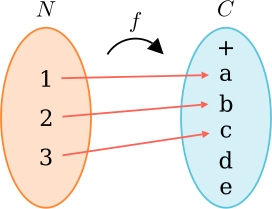
\includegraphics[height=3.5cm]{images/part-1/functions/character-of.png}
        \caption{Arrow Diagram of $f$}
    \end{figure}

    For $f$, we see that
    \begin{itemize}
        \item its domain is $N$;
        \item its codomain is $C$; and
        \item its range is $\{\text{a}, \text{b}, \text{c}\}$.
    \end{itemize}
\end{example}

\begin{example}[The Successor Function]
    Let's look at the successor function restricted to the natural numbers again, i.e. the function $S: \N \to \N$. We can draw an arrow diagram for this function.
    \begin{figure}[H]
        \centering
        
\includegraphics[height=3.5cm]{images/part-1/functions/successor.png}
        \caption{Arrow Diagram of $S$}
    \end{figure}

    We see that
    \begin{itemize}
        \item its domain is $\N$;
        \item its codomain is also $\N$; and
        \item its range is $\N \setminus \{0\}$.
    \end{itemize}
\end{example}

% TODO: Add exercise for domain, codomain, and range

\section{Axiom Schema of Replacement}  % aka Axiom of Replacement
TODO: Add

\section{Well-Defined Functions}
TODO: Add
% Introduce what happens when a function's rule is not OK

\section{Injections, Surjections, Bijections}
TODO: Add
% Introduce injectivity
% Introduce surjectivity
% Introduce bijectivity
% Introduce inverse functions (for bijective functions)

\section{Composition of Functions}
TODO: Add
% Give an idea of what function composition process is like (e.g., as machines feeding into each other)
% Define function composition
% Give result of composition with identity function
% Give result of composition with inverse
% Give result of composition with injections and surjections
